\documentclass[a4j,fleqn,dvipdfmx,uplatex]{jsarticle}

\usepackage{sice-si}

\usepackage{epic,eepic}
\usepackage[dvipdfmx]{graphics}
\usepackage[dvipdfmx]{graphicx}
\usepackage[dvipdfmx]{color}
% \usepackage{fancyhdr} % ヘッダフッタの罫線と文字出力
% \pagestyle{fancy} % ヘッダフッタの罫線と文字出力(fancyhdrパッケージとセット)
\usepackage{amsmath} % 数式用
\usepackage{amssymb}
\usepackage{tabularx}
\usepackage{enumerate}
\usepackage{txfonts}
\usepackage{url}
\usepackage{pdflscape}
% \usepackage{bm}
\usepackage[subrefformat=parens]{subcaption}
\captionsetup{compatibility=false}

% 図表参照に章番号付加 章をまたいでの参照は不可
\newcommand{\figref}[1]{Fig.\ \ref{#1}}
\newcommand{\tableref}[1]{Table.\ \ref{#1}}

% 章番号の後調整
\newcommand{\secref}[1]{\ref{#1}\hspace{0.2zw}章}
% 節番号の後調整
\newcommand{\subsecref}[1]{\ref{#1}\hspace{0.2zw}節}


\begin{document}
%
% タイトルと著者名
\title{FTE新入社員課題報告書\\[1.5mm]本社屋上室外機における散水システム導入と\\省エネ効果に対する実験的検証} % 和文タイトル
\name{○高橋 京佑, 小坂 丞, 仲野 茂翠, 設樂 日和, 𠮷岡 拓海, 渡辺 夏芽, 
\\中村 天音, 塚田 浩貴, 青木 昇, 吉川 唯希, 佐藤 央都, 阪田 悠} % 著者名

\etitle{Introduction and Experimental verification on its energy-saving effect \\of Watering System for Condensing Unit on the office rooftop} % 英文タイトル
\ename{\small○KEISUKE Takahashi, TASUKU Kosaka, MOTOAKI Nakano, HINOWA Shidara, TAKUMI Yoshioka, NATSUME Watanabe, \\
AMANE Nakamura, HIROTAKA Tsukada, NOBORU Aoki, ITSUKI Yoshikawa, HIROTO Sato, YU Sakata}	%著者名(英)
%%%%%%%%%%%%%%%%%%%%%%%%%%%%%%%%%%%%%%%%%%%%%%%%%%%%%%%%%%%%%%%%%%%%%%%%%%%%%%%%%%%%%%%%%%%%%%%%%%%
% アブストラクト
% \abst{}

% タイトルの出力
\maketitle
%%%%%%%%%%%%%%%%%%%%%%%%%%%%%%%%%%%%%%%%%%%%%%%%%%%%%%%%%%%%%%%%%%%%%%%%%%%%%%%%%%%%%%%%%%%%%%%%%%%
% 本文
\section{序論}\label{sec1}
\subsection{背景}\label{background}
近年, 地球温暖化の影響のため, 日本全国の気温は上昇傾向にあり, 
2021年の大阪府の年間平均気温は1883年に比べ2.5℃上昇している\cite{temp_osaka}. 
さらに, 2021年の真夏日と猛暑日の合計日数は, 2014年の65日に比べ13日増加, 
猛暑日に関しては8日増加しており\cite{temp_osaka2}, 1880年からの真夏日および
猛暑日の長期的推移を見ると増加傾向である (\figref{fig1:temp_osaka}). 

\begin{figure}[htb]
  \centering
  \begin{minipage}[b]{\linewidth}
      \centering
      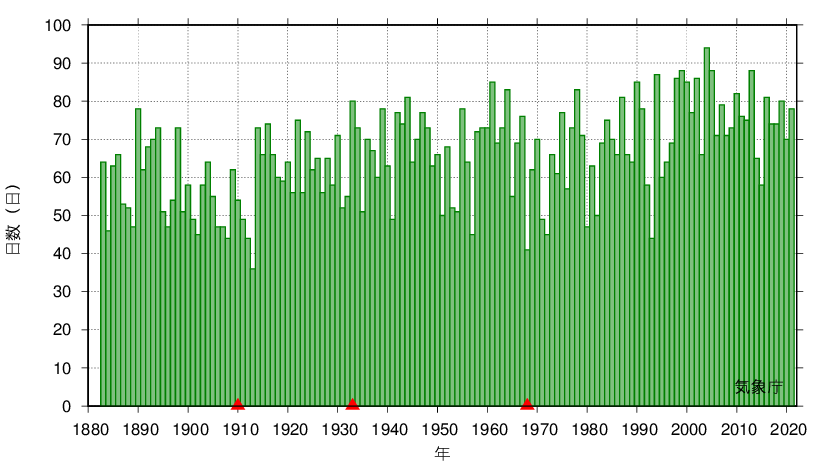
\includegraphics[width=\linewidth]{img/OSAKA_tmaxGE30.png}
      \subcaption{大阪 真夏日}
      \label{subfig1:temp_osaka}
    \end{minipage}\\
    \begin{minipage}[b]{\linewidth}
      \centering
      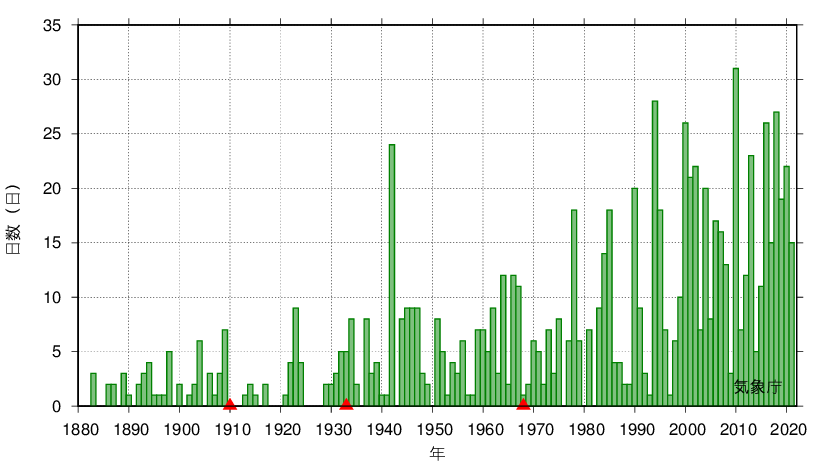
\includegraphics[width=\linewidth]{img/OSAKA_tmaxGE35.png}
      \subcaption{大阪 猛暑日}
      \label{subfig1:temp_osaka2}
    \end{minipage}
    \caption{真夏日および猛暑日の年間日数 1883-2021年\cite{temp_osaka3}}
    \label{fig1:temp_osaka}
\end{figure}
 
気温上昇に伴う問題点として, 空調による電力量の増加が懸念される. 
一般に空調機器は室内機と室外機に構成されており, 
冷房時において, 室外機は冷媒の圧縮・凝縮, 室内機は蒸発・膨張の過程をそれぞれ担っている. 
室外機は高圧化した冷媒ガスを外気と熱交換させることで凝縮させ, 
室内機では, 膨張した冷媒液を室内の空気と熱交換させて冷媒の潜熱を利用して冷却する. 

ここで, 室外機吸い込み側空気, つまり外気の温度が上昇すると, それに付随して凝縮温度
が高くなる. それにより凝縮負荷が大きくなり, 圧縮機の駆動力が占める比率が大きくなるため, 
結果的に成績係数が小さくなる. したがって, 同じ冷却能力を出すためには消費電力が大きくなる.  
さらに, 空冷機の冷却温度は外気温度マイナス10$^\circ$Cが目安とされており, 猛暑日になると
室内が十分に冷えなくなる可能性や高圧化防止のため運転が停止される問題もある. 

これらの問題を防止するために凝縮器の熱交換促進技術が様々考えられており, 特に
自動散水機の導入が挙げられる. 過去に散水装置を導入した食品メーカーの経済効果試算では
使用電力量は約7\%, 電気料金は約13\%の削減率が見込める結果となっている\cite{thesis3}. 

そこで, 実際に散水効果を検証するため, 室外機凝縮器部分にバケツを用いて散水をし, 
その電力量を計測した. 計測は本社2階北側のユニットクーラー用の室外機1台を用い, 
散水の有無による電力量の比較を行った. その際の計測環境は\tableref{table:ex1}に示す. 
\figref{fig1:compare_watering}に示すように, 実験2 (散水あり) の電力量は実験1 (散水なし) のそれと
比較して小さくなっていることが分かる.

\begin{table}[htb]
  \caption{計測環境}
  \label{table:ex1}
  \centering
  \begin{tabular}{lcccc}
     & 外気温 & 湿度 & 設定温度 & 気候 \\[-1.5mm]
     & [$^\circ$C] & [\%] & [$^\circ$C] &  \\
    \hline \hline
    実験1 & 34.3 & 48.0 & 27.0 & 晴れ  \\
    実験2 & 32.9 & 58.9 & 27.0 & 曇り \\
    \hline
  \end{tabular}
\end{table}

\begin{figure}[htb]
  \centering
      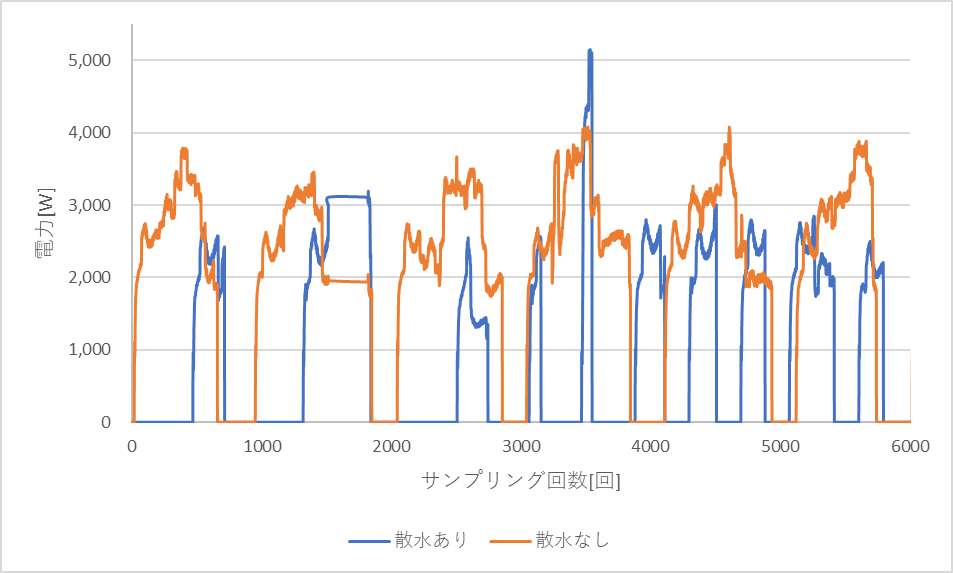
\includegraphics[width=\linewidth]{img/ex1.png}
      \caption{散水の有無による電力量比較\\ \small ※ サンプリング周波数=1Hz}
      \label{fig1:compare_watering}
\end{figure}


\subsection{目的}\label{purpose}
\subsecref{background} より, 室外機において散水装置の導入が電力量低減の効果
があるのではないかと考えられる. 
そこで本研究では, 散水システムの導入に伴い自作の散水装置を組み上げ, 
天候や室内設定温度など様々な条件下で比較検証を行い, 
電気代および水道代とのコストバランスを考慮に入れ, 最適な散水条件を検討することを
目的として実験を行った. 

\section{計測実験}\label{sec2}
\subsection{計測対象と実験方式}
本研究で調査対象とした室外機はビル用マルチエアコンである三菱社 
PUHY-EP335DMG9 \cite{condensing_unit}を採用した (\figref{fig:condensing_unit}, \tableref{table:hard}). 
この室外機に散水の有無および散水方法など変更した以下の4条件に分けて計測を行っていく.  

\begin{description}
  \item[  実験1 ] 散水なし
  \item[  実験2 ] 離散散水 (手動)
  \item[  実験3 ] 継続散水 (自作散水システム)
  \item[  実験4 ] 離散散水 (自作散水システム)
\end{description}

\begin{figure}[htb]
  \centering
  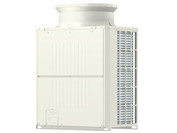
\includegraphics[width=0.7\linewidth]{img/PUHY-EP335DMG9.jpg}
  \caption{室外機 PUHY-EP355DMG9}
  \label{fig:condensing_unit}
\end{figure}

\begin{table}[htb]
  \caption{室外機仕様(冷房時)}
  \label{table:hard}
  \centering
  \begin{tabular}{lr}
    PUHY-EP355DMG9 & \\
    \hline \hline
    電源 & 3相 200V \\
    能力 & 33.5 kW \\
    消費電力 & 10.7 kW \\
    冷媒 & R410 \\
    \hline
  \end{tabular}
\end{table}

実験で計測するパラメータは以下の通りである. 

\begin{itemize}
  \item 外気環境(気温, 相対湿度, 風速)
  \item 凝縮器入口温度 (2箇所)
  \item 凝縮器出口温度 (2箇所)
  \item 室外機 (圧縮機運転状況)
  \item 電気系 (電流, 電圧, 電力量)
  \item 散水系 (水温, 散水流量)
  \item 室内系 (設定温度, 温度, 湿度)
\end{itemize}

また、計測時間は13時から15時までの2時間とし, 
データログを取れるもの以外のパラメータは10分ごとに計測するとした. 
計測で得られた値を各実験で比較し考察していく. 

\subsection{自作散水システム}
本節では, 計測実験の比較対象として自作する散水システムの概要について説明する.

屋上にある蛇口からホースと塩化ビニル管を結合させて室外機まで通し, 散水ノズルを
凝縮器側に左右3個ずつ計6個を設置した(\figref{fig2:watering_sys}). 
尚, 同システムの系統図は\figref{fig:w_s_flow}に示す. 

\begin{figure}[htb]
  \centering
    \begin{minipage}[b]{0.45\linewidth}
      \centering
      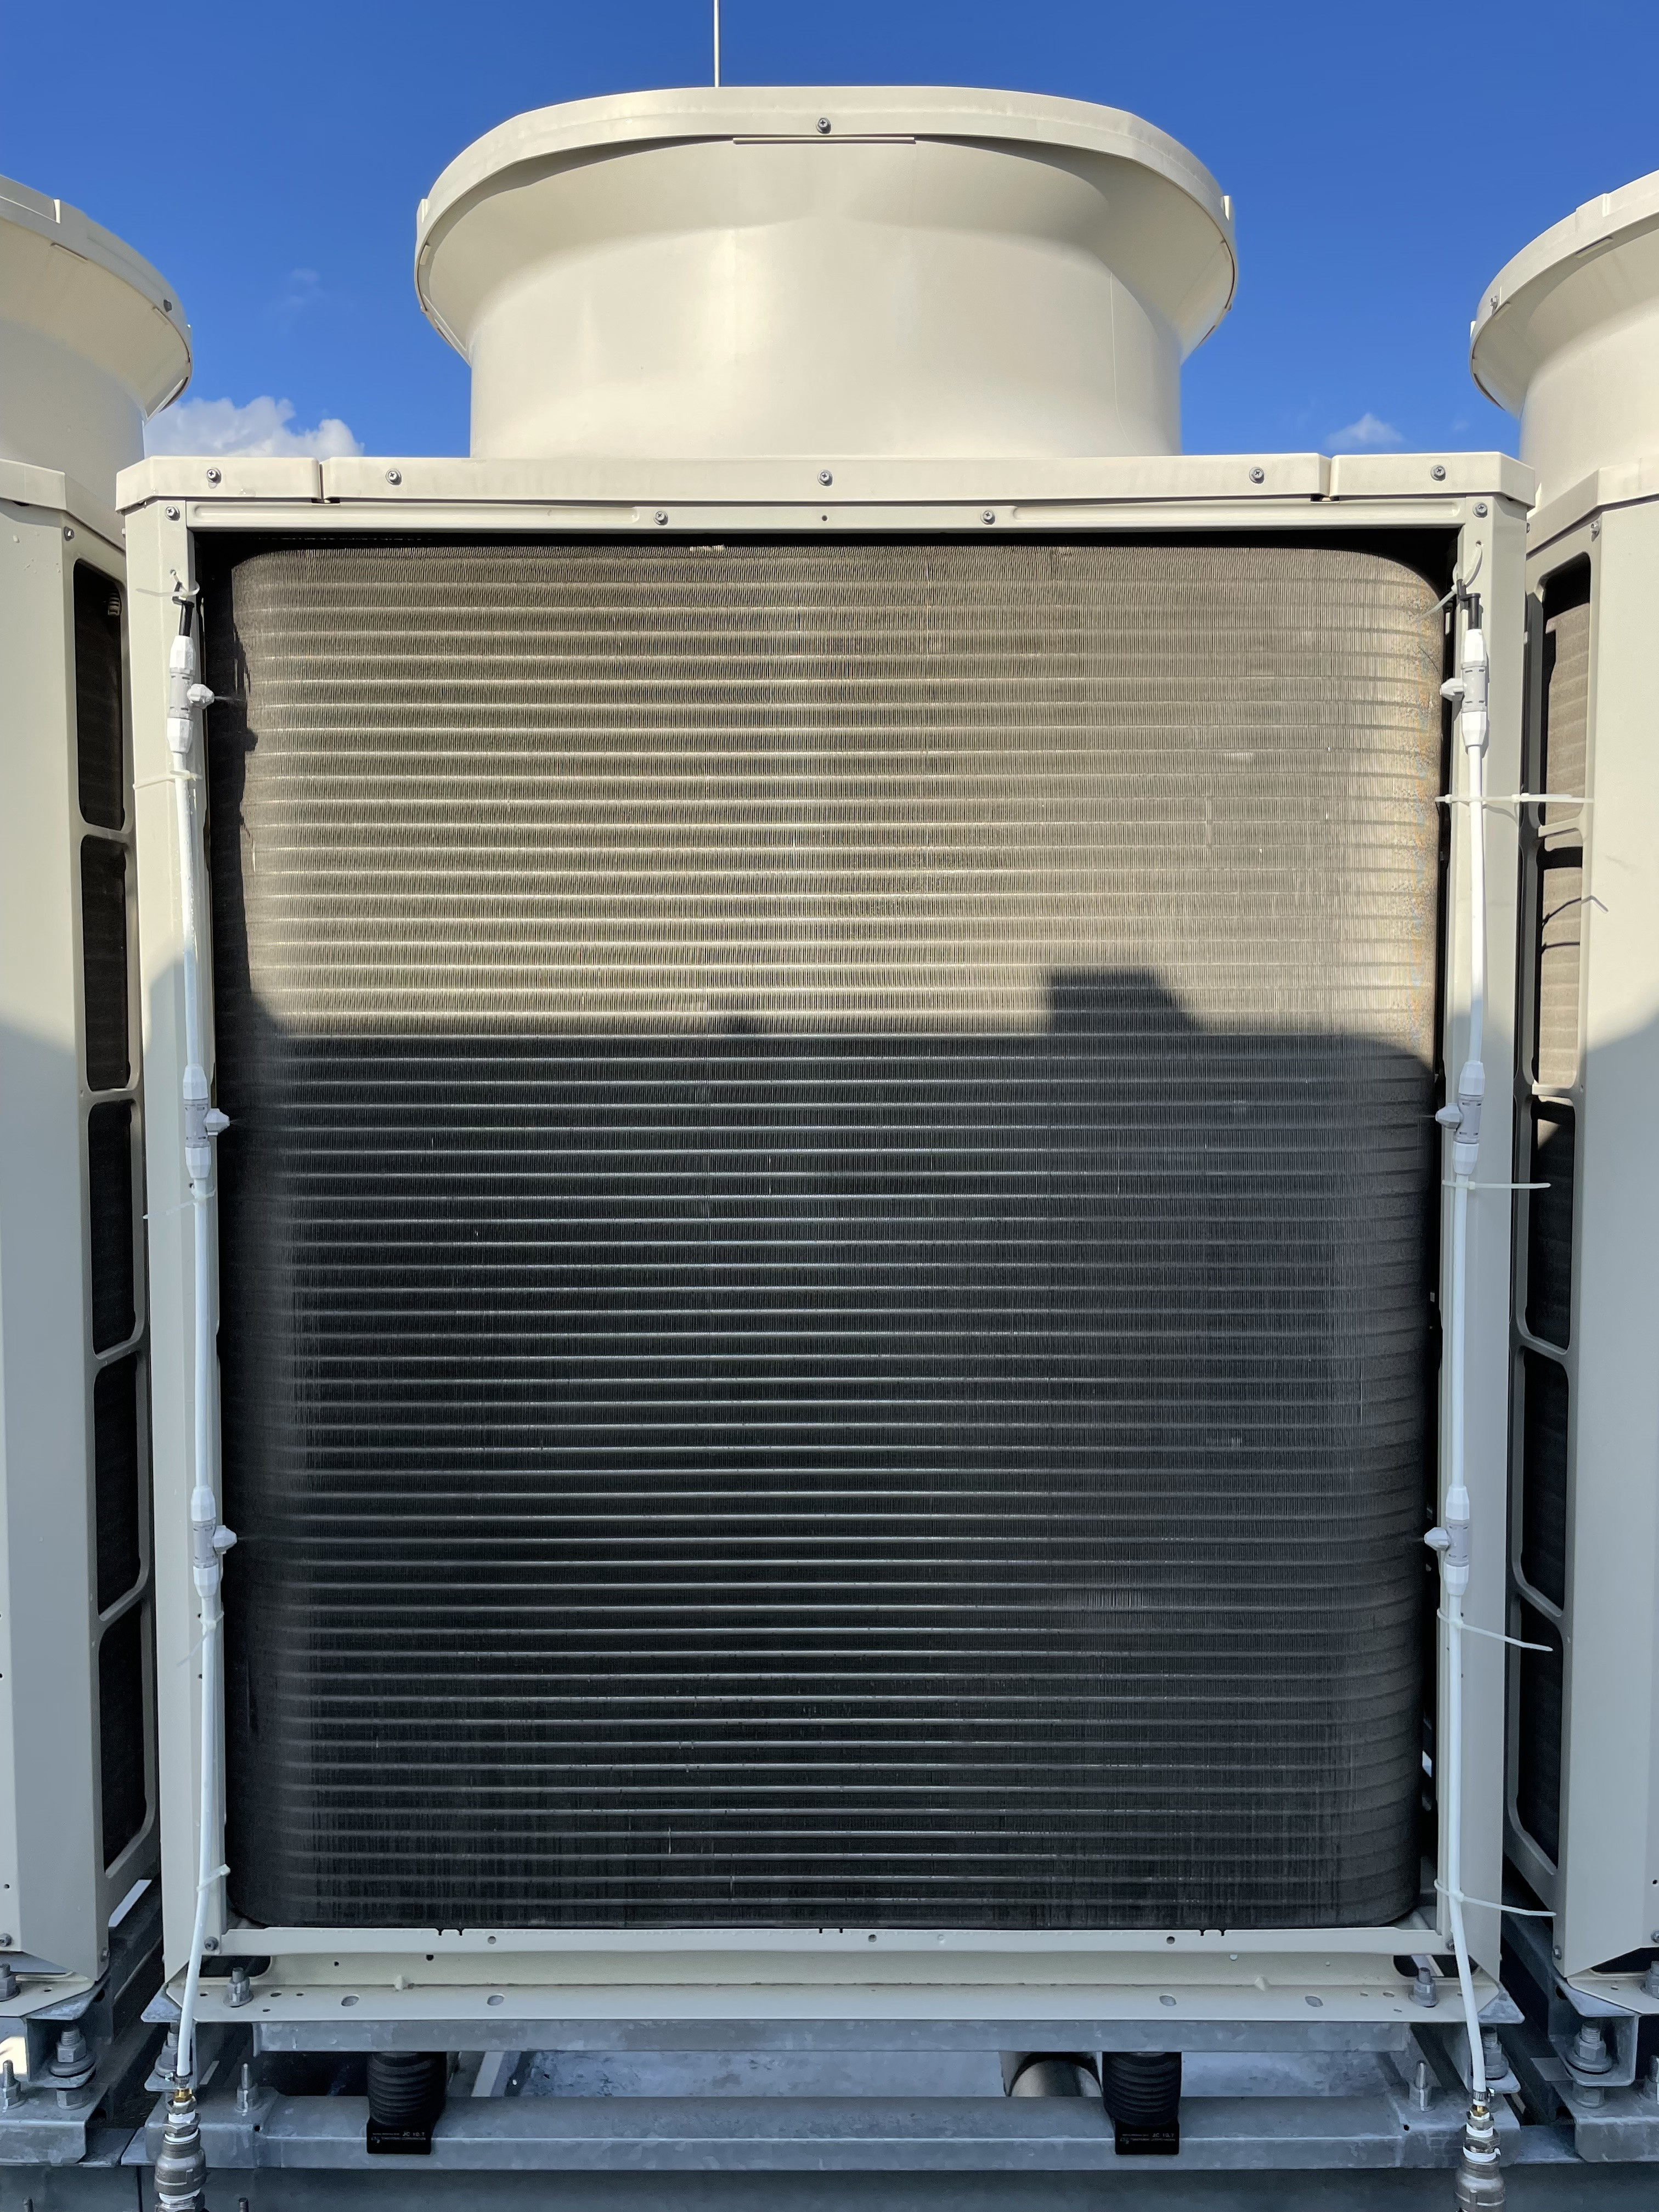
\includegraphics[width=\linewidth]{img/IMG_0146.jpg}
      \subcaption{凝縮器側散水部}
    \end{minipage}
    \begin{minipage}[b]{0.45\linewidth}
      \centering
      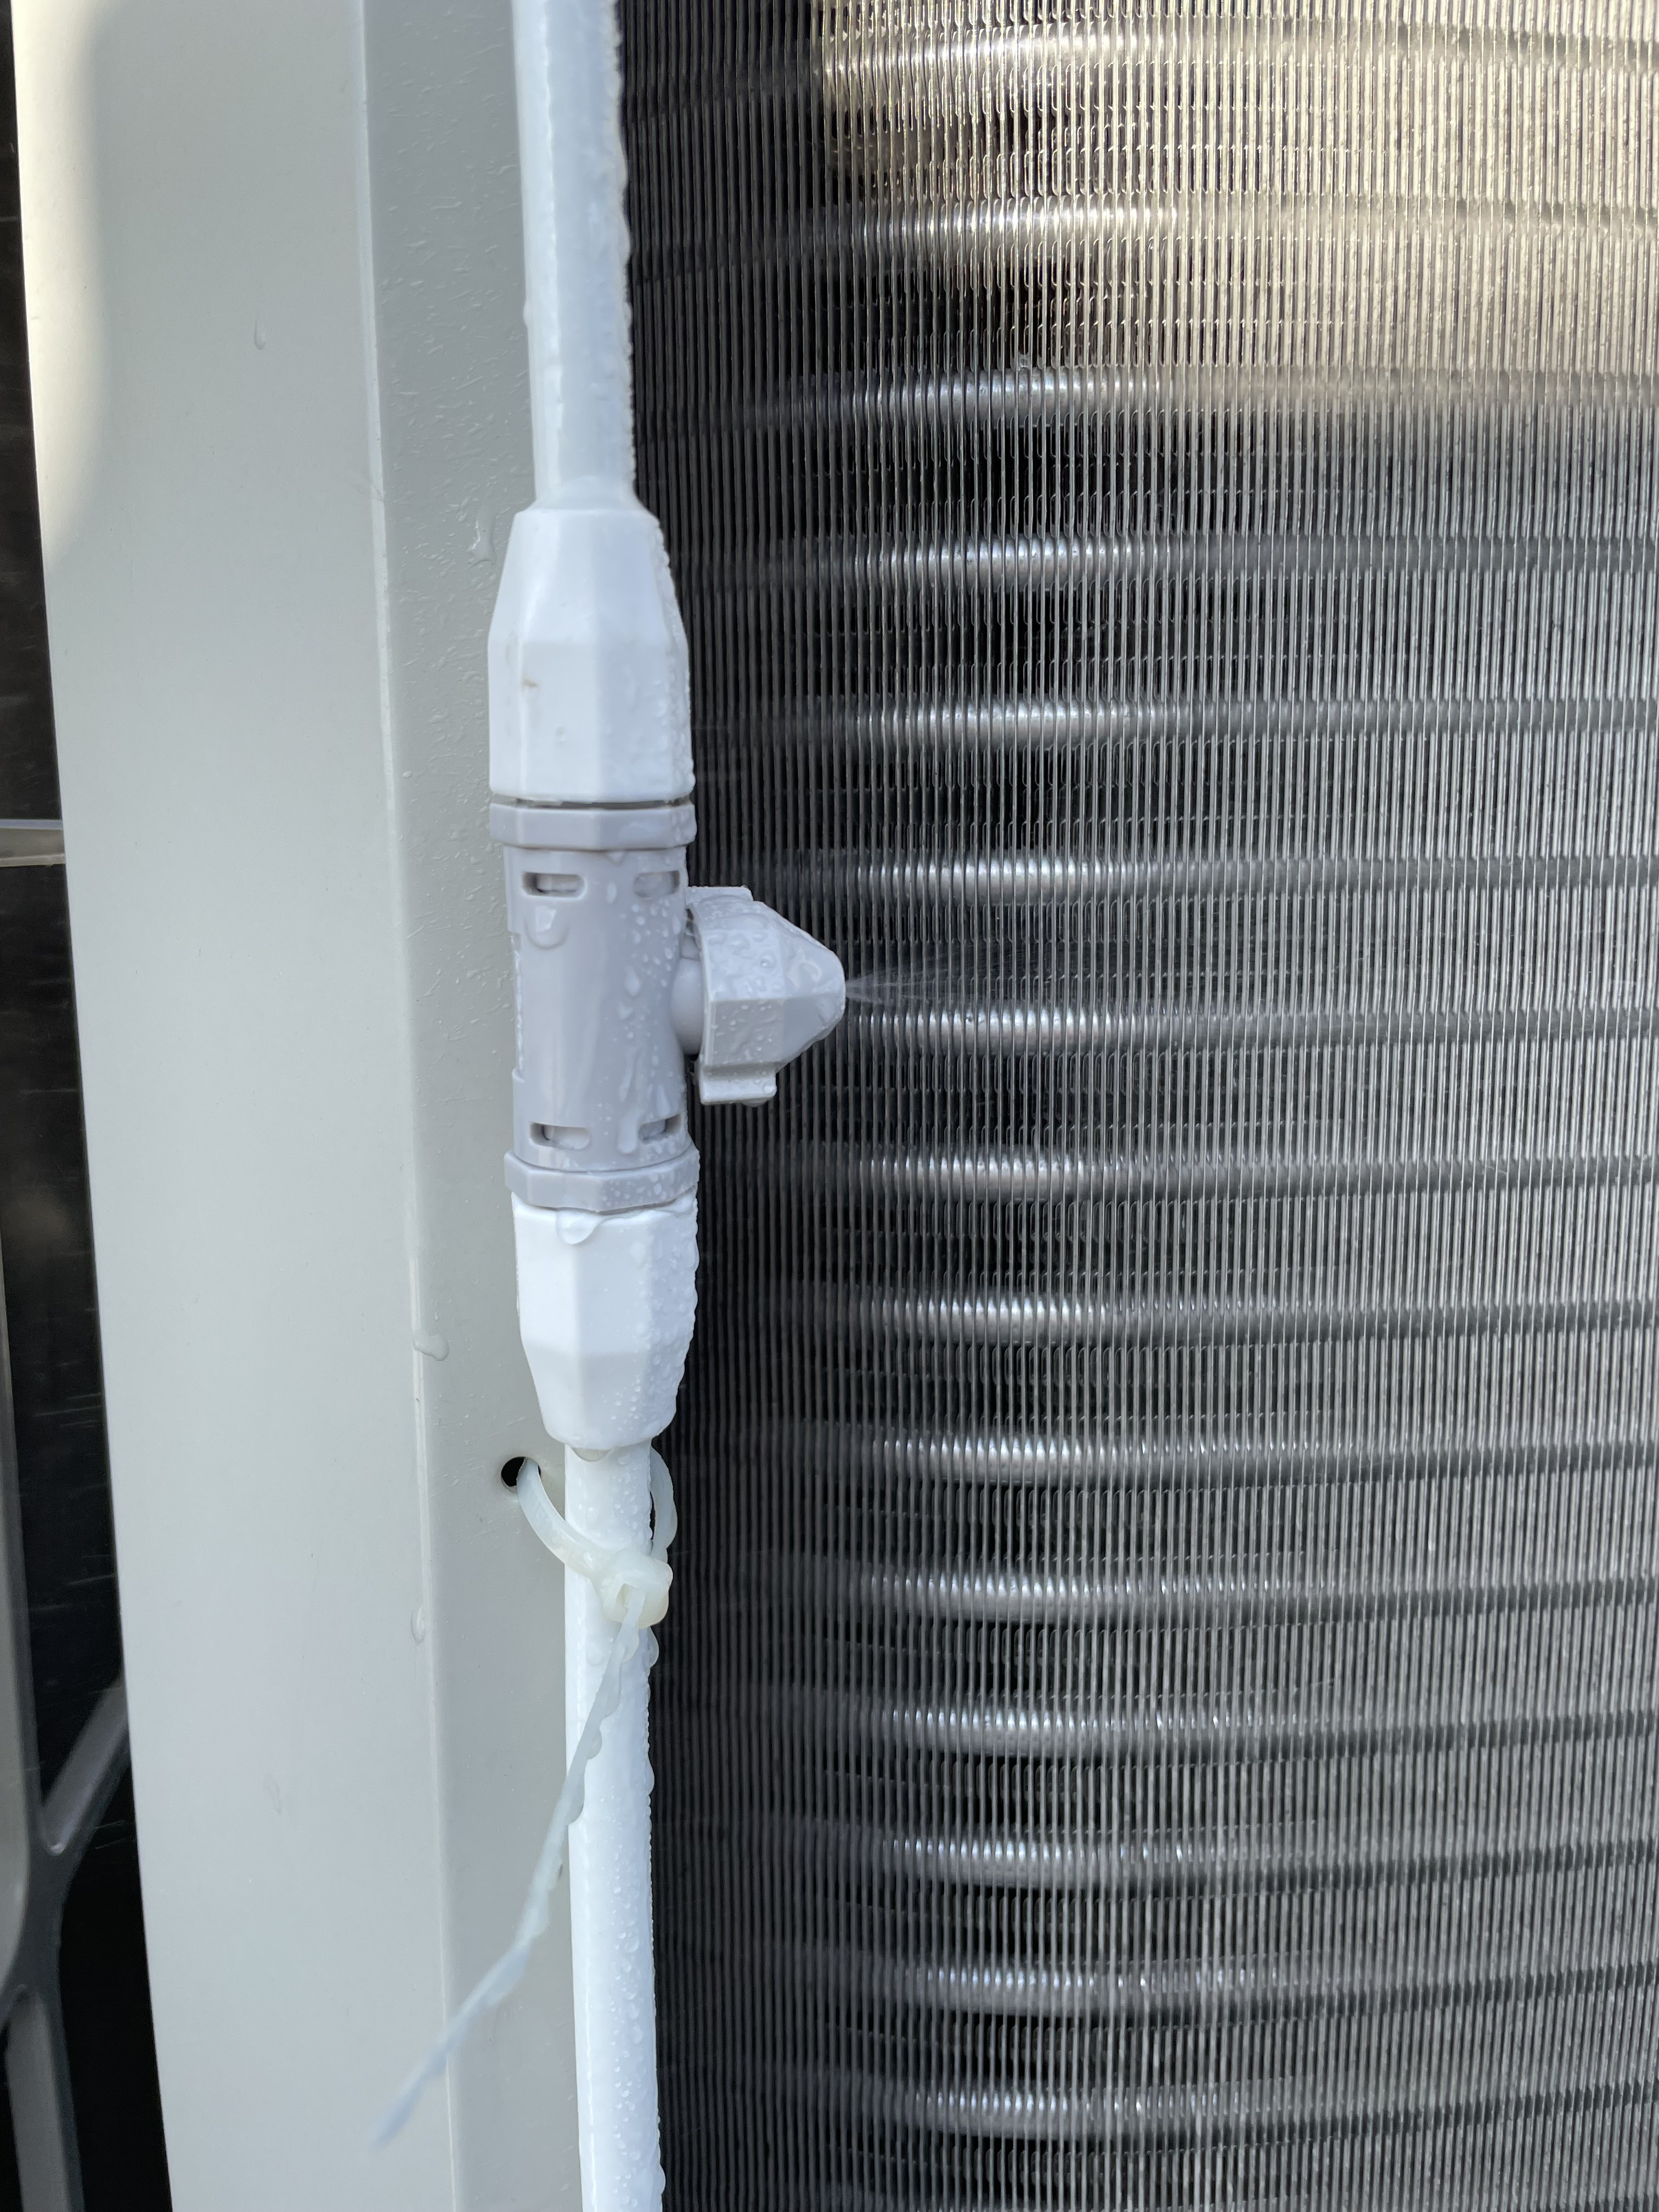
\includegraphics[width=\linewidth]{img/IMG_0142.jpg}
      \subcaption{散水用ノズル}
    \end{minipage}
  \caption{散水システム}
  \label{fig2:watering_sys}
\end{figure}

\begin{figure}[htb]
  \centering
  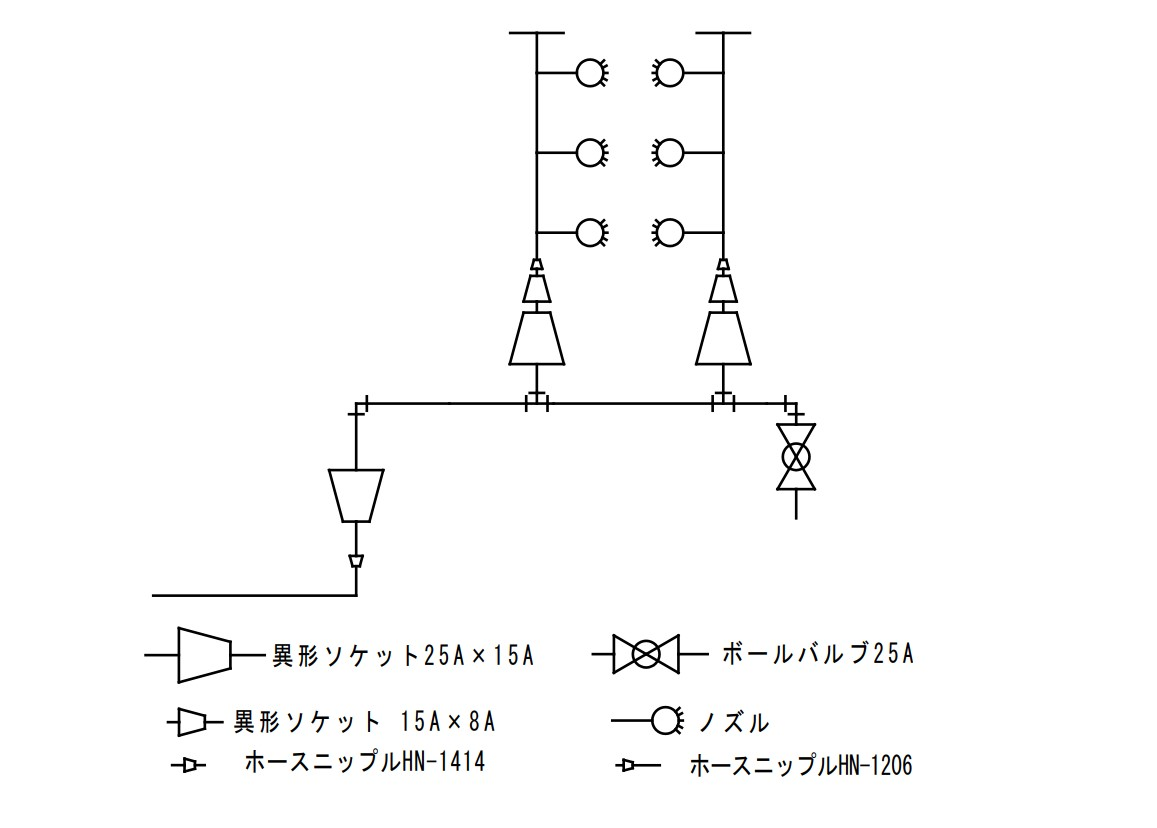
\includegraphics[width=\linewidth]{img/flow.jpg}
  \caption{自作散水システムの系統図}
  \label{fig:w_s_flow}
\end{figure}

\section{結果}\label{sec3}
各計測日における環境および結果, 従量電気料金を25円として見積もった際の
各実験における2時間でかかった電気代, 計測時間に対する電力量の推移
はそれぞれ\tableref{table:ex}, \figref{fig:fee}, \figref{fig:ex_outputs_1/2}に示す. 

\begin{table*}[htb]
  \caption{実験の計測環境及び結果}
  \label{table:ex}
  \centering
  \begin{tabular}{lrrrrrrrrrrrr}
    計測日 & 散水方式 & 気温 & 湿度 & 外気h & 気候 & 設定温度 & 消費電力 & 電気代 & 変化率 \\[-1.5mm]
     & & \small [$^\circ$C] & \small [\%] & \small [kJ/kg] & & \small [$^\circ$C] & \small [kWh] & \small [円] & \small [\%]\\
    \hline \hline
    7/13 & 散水なし & 34.3 & 48.0 & 76.5 & 晴れ & 26 - 27 & 4.24 & 100 & ― \\
    7/15 & 手動散水(T=30,90) & 32.9 & 58.9 & 80.9 & 曇り & 27.0 & 1.66 & 42 & -58 \\
    7/19 & 散水なし & 27.9 & 82.8 & 78.4 & 雨 & 27.0 & 2.88 & 75 & -25 \\
    7/21 & 手動散水(T=30,90) & 32.1 & 58.4 & 77.5 & 曇り/雨 & 27.0 & 1.04 & 26 & -74 \\[3mm]
    7/23 & 継続散水(T=30-120) & 33.2 & 43.4 & 66.2 & 晴れ & 27.0 & 0.72 & 18 & -82 \\
    7/25 & 継続散水(T=30-120) & 36.5 & 42.2 & 78.5 & 晴れ & 25.0 & 3.12 & 79 & ― \\
    7/26 & 継続散水(T=30-120) & 37.5 & 41.0 & 80.6 & 晴れ & 25.0 & 4.45 & 111 & +40 \\
    7/28 & 継続散水(T=0-30, 60-70) & 37.0 & 47.0 & 85.2 & 晴れ & 25.0 & & 84 & +6\\
    7/29 & 離散散水(T=30-120:20分) & 36.0 & 45.0 & 79.6 & 晴れ & 25.0 &  & 94 & +18 \\
    % 8/1  &  & 35.3 & 51.1 & 83.0 & 晴れ & 25.0 & & & \\
    8/03  & \footnotesize 離散散水(T=30-70:10分, 95-120:5分) & 35.6 & 49.7 & 82.7 & 晴れ & 25.0 &  & 41 & -48 \\
    \hline
  \end{tabular}\\
  \small ※ h : 比エンタルピー, T : 計測時間[min]
\end{table*}

\begin{figure}[htb]
  \centering
  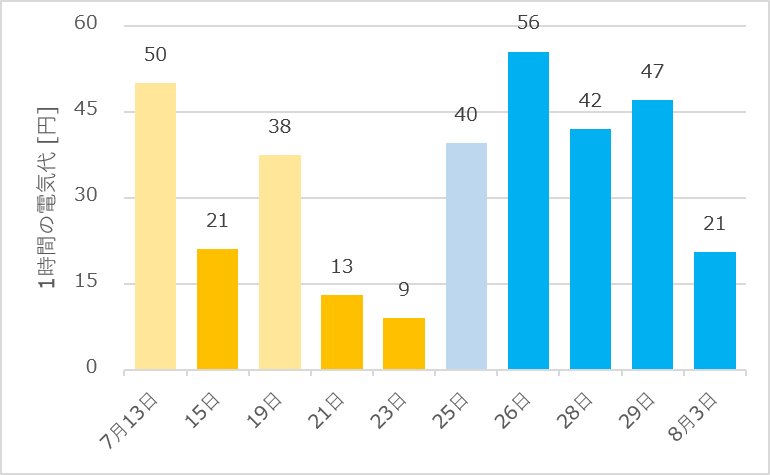
\includegraphics[width=\linewidth]{img/fee.png}
  \caption{電気料金比較\\ \small 橙: 設定温度27℃, 青: 設定温度25℃}
  \label{fig:fee}
\end{figure}

\begin{figure*}[htb]
  \centering
  \begin{subfigure}[t]{0.32\linewidth}
    \centering
    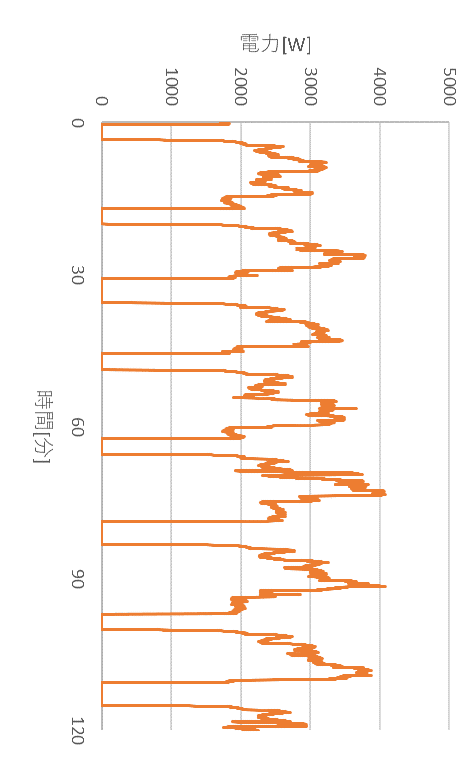
\includegraphics[width=\linewidth]{img/0713_power.png}
    \caption{7/13 散水なし}\label{fig:a}
  \end{subfigure}
  \begin{subfigure}[t]{0.32\linewidth}
    \centering
    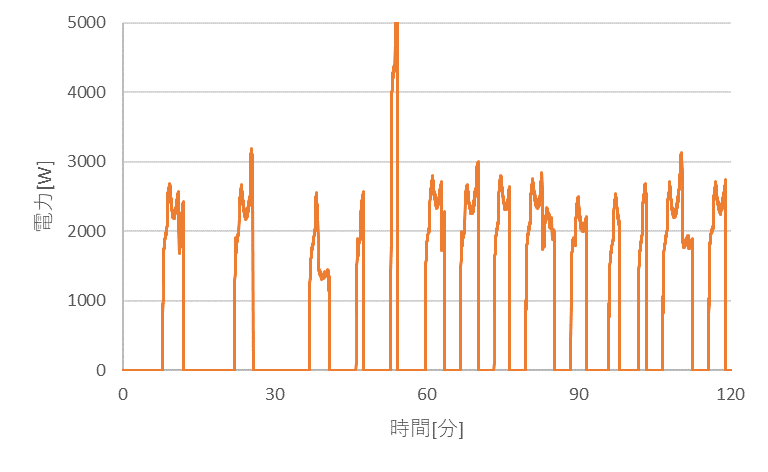
\includegraphics[width=\linewidth]{img/0715_power.png}
    \caption{7/15 1分散水\\(T=30, 90)}\label{fig:b}
  \end{subfigure}
  \begin{subfigure}[t]{0.32\linewidth}
    \centering
    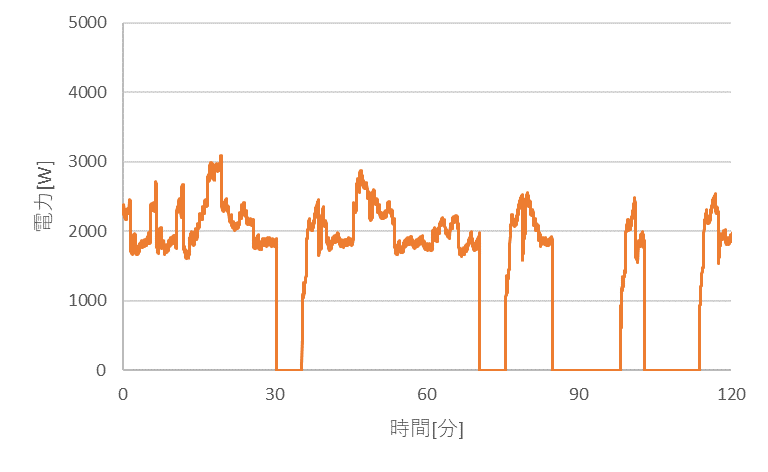
\includegraphics[width=\linewidth]{img/0719_power.png}
    \caption{7/19 散水なし\\(雨天)}\label{fig:c}
  \end{subfigure}\\
  \begin{subfigure}[t]{0.32\linewidth}
    \centering
    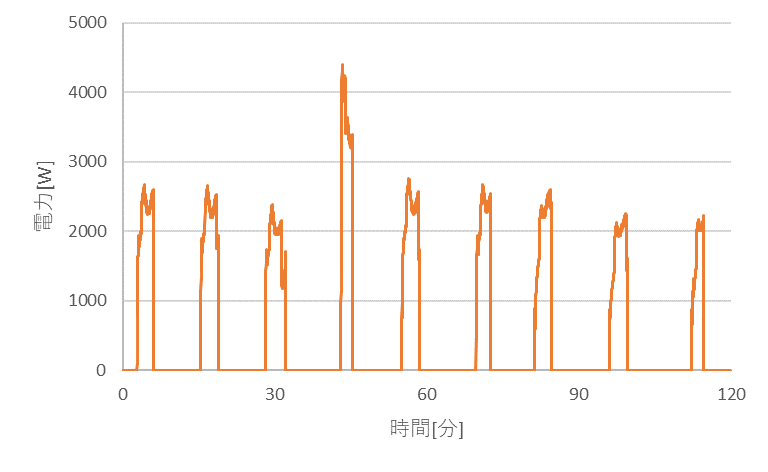
\includegraphics[width=\linewidth]{img/0721_power.png}
    \caption{7/21 手動散水\\(T=30, 90)}\label{fig:d}
  \end{subfigure}
  \begin{subfigure}[t]{0.32\linewidth}
    \centering
    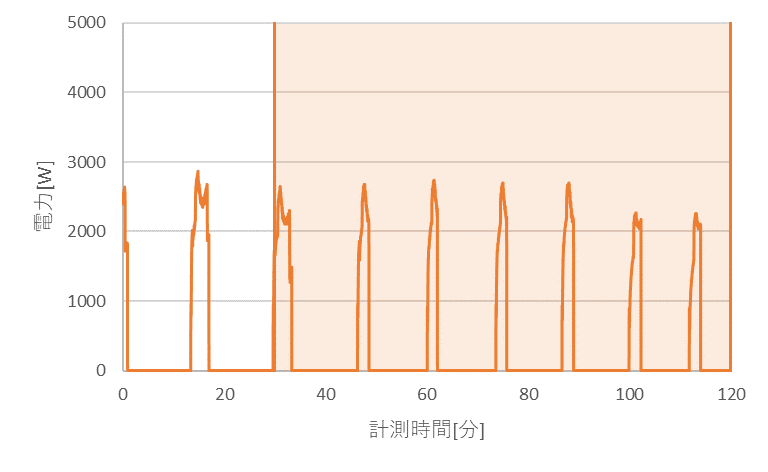
\includegraphics[width=\linewidth]{img/t_p/20220723.png}
    \caption{7/23 継続散水\\(T=30 - 120)}\label{fig:e}
  \end{subfigure}
  \begin{subfigure}[t]{0.32\linewidth}
      \centering
      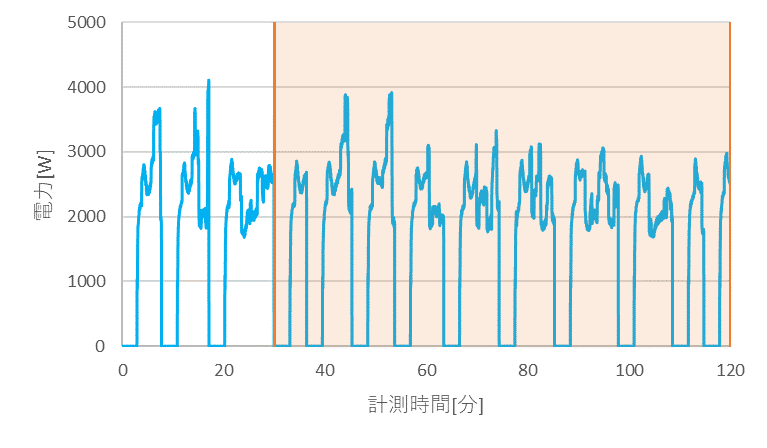
\includegraphics[width=\linewidth]{img/t_p/20220725.png}
      \caption{7/25 継続散水\\(T=30 - 120)}\label{fig:f}
  \end{subfigure}
  \caption{電力量推移と散水タイミング(1 of 2) \\ \small 橙:設定温度27℃, 青:設定温度25℃, T:計測時間[分]}\label{fig:ex_outputs_1/2}
\end{figure*}

\begin{figure*}[htb]
  \addtocounter{figure}{-1}
  \centering
  \begin{subfigure}[t]{0.32\linewidth}
    \addtocounter{subfigure}{6} % 最初のsubfigure数
    \centering
    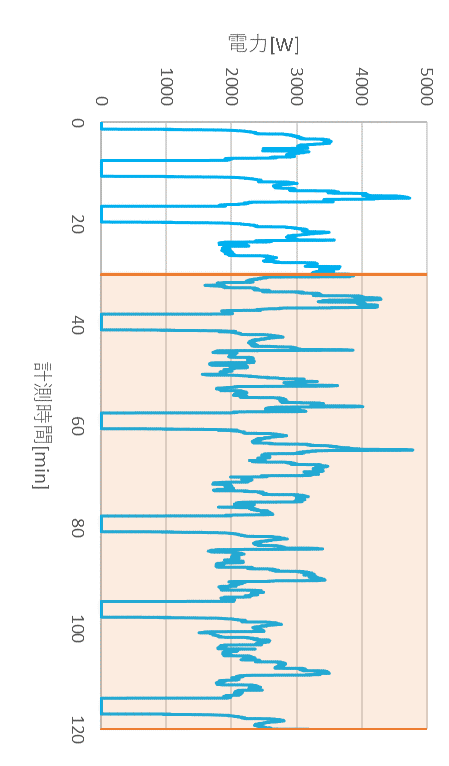
\includegraphics[width=\linewidth]{img/t_p/20220726.png}
    \caption{7/26 継続散水\\(T=30 - 120)}\label{fig:g}
  \end{subfigure}
  \begin{subfigure}[t]{0.32\linewidth}
    \centering
    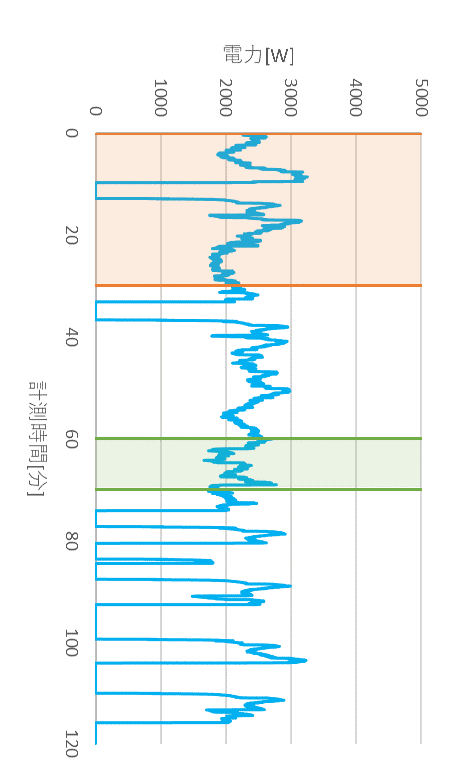
\includegraphics[width=\linewidth]{img/t_p/20220728.png}
    \caption{7/28 継続散水\\(T=0 - 30, 60 - 70)}\label{fig:h}
  \end{subfigure}\\
  \begin{subfigure}[t]{0.32\linewidth}
    \centering
    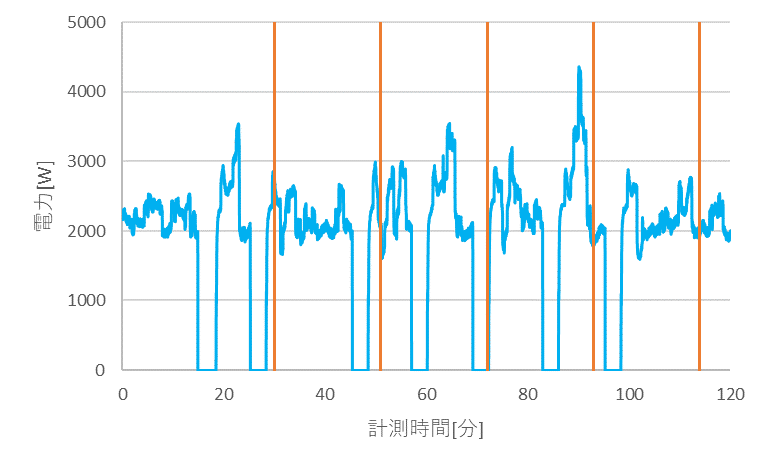
\includegraphics[width=\linewidth]{img/t_p/20220729.png}
    \caption{7/29 1分散水\\(T=30- 120: 20min)}\label{fig:i}
  \end{subfigure}
  \begin{subfigure}[t]{0.32\linewidth}
    \centering
    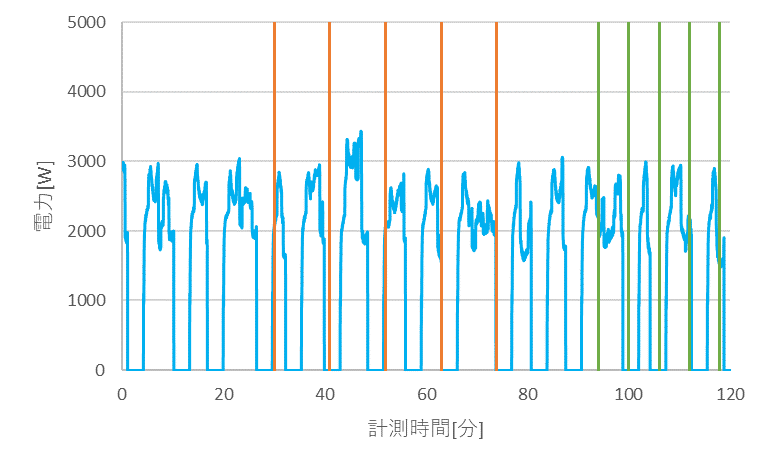
\includegraphics[width=\linewidth]{img/t_p/20220803.png}
    \caption{8/3 1分散水\\ \small (T=30-90:10min, 90-:5min)}\label{fig:j}
  \end{subfigure}
  \caption{電力量推移と散水タイミング(続き)\\ \small グラフ内縦線は1分散水時の時刻, 背景色付き面は継続散水を表す}\label{fig:ex_outputs_2/2}
\end{figure*}

\figref{fig:b}と\figref{fig:d}を比較すると, 散水直後の電力ピークが低下し, その後
段階的に増加していることがわかる. 一方, \figref{fig:a}や\figref{fig:c}
は電力ピークの大きな増減は見られない. また, \figref{fig:c}では計測開始から
90分程度まで天候は雨であったが, その間, 圧縮機が長時間運転をしていることがわかる. 
ただし, 90分以降に雨が止み蒸発熱によって凝縮器温度が低下し熱交換が促進されたものだと考察できる. 
自作装置による散水は, 継続散水の場合は電力量の大幅な低下は見られなかった. 一方, 散水方法を継続的
から\figref{fig:i}や\figref{fig:j}のように離散的な方式に変更すると, 圧縮機の発停時間が小さくなり, 
電力ピークも小さくなった. 

さらに, \figref{fig:fee}に示すように, 設定温度が27℃の場合は散水時に大幅な電気料金の削減ができた. 
一方, 設定温度が25℃の場合は27℃の場合との相関は取れなかった. しかし, \figref{fig:i}や
\figref{fig:j}に示すように, 散水後の電力量最大値は設定温度27℃の場合と同じく
小さくなる傾向になった. 



\section{考察}\label{sec4}
\figref{fig:fee}から, 晴天時散水なしの場合と比べた消費電力の減少率は, 手動散水の場合で約60\%, 
雨天時散水なしで約32\% 減少することが分かった. 
これらの値は外気環境が異なるため, 正当性の評価としては難しいが, 傾向として凝縮器が濡れることにより
電力量が減少していることが分かる. 

また, 散水ありの場合でも, 手動で行った場合と自動機器を用いて散水した場合では, 
散水ノズルがフィンに対して垂直に配置していることから, 手動よりも水がフィンの奥まで
入りこまない可能性があるため, 以下ではそれぞれの散水効果の比較を考える. 
\figref{fig:b}から、手動での散水では, 散水直後での室外機の発停間隔が短くなり, 
水の潜熱による短時間運転を実現している一方で, 散水後30分以降については, 散水前よりも
運転時間が長い. これは、実験で用いた室外機のフィン間隔が1.4 ㎜という狭さのために, 
伝熱面に残った数mmスケールの水滴が蒸発しきらずに残り続け, 伝熱面積の減少及び室外ファンの
風を遮り, 運転時間の増大につながったのではないかと考えられる.
次に\figref{fig:e}から, 散水前後において露骨な電力量の減少がみられる, これは, 水の潜熱
による短時間運転を実現しており, 手動散水よりも電力量の減少が効果的に行われている
と考えられる.
以上の議論から, より効率よく潜熱を用いた熱交換をするには, なるべく水滴を作らないように散水を連続的に行うのではなく, 
断続して行い, フィン面に付着した水がある程度蒸発するための時間を設ける必要があると考えられる.

ここで, 断続的な散水には散水の継続時間と再び散水する周期が必要である. \figref{fig:h}から, 散水継続時間はより
短いほうが電力量が抑えられるという結果となった. これも先述した水滴による効率悪化
であると考えられる. \figref{fig:e}ではその効果が見られないのは, 設定温度を7/28
では27℃から25℃に下げ, より熱負荷が大きくなり, 熱交換の効率がより求められるように
なったと考えられる. 
また,散水周期に関しては\figref{fig:i},\figref{fig:j}から,周期を小さくすることにより,
発停周期についても小さくなると考えられる. 
尚,\figref{fig:i}の70分, 95分頃に現れた急激なピークは, 凝縮器表面に付着した水が
すべて蒸発し, 熱交換の効率が急激に悪化したため, 冷媒循環量を上げて熱交換するよう
圧縮機の出力が上がったと考えられる. すなわち, 気温35℃, 湿度40\%の環境では散水周期は
10~15分以下であると考えられる. 

以下では電気力量を算出し,散水効果の度合いについて数値的に求める.\figref{fig:j}から,
室外機の運転時間と停止時間を一組と考え,その時間における平均電力を求めた.
\figref{fig:8/3_sato}に各運転時間における平均電力を示す.

\begin{figure}[htb]
  \centering
  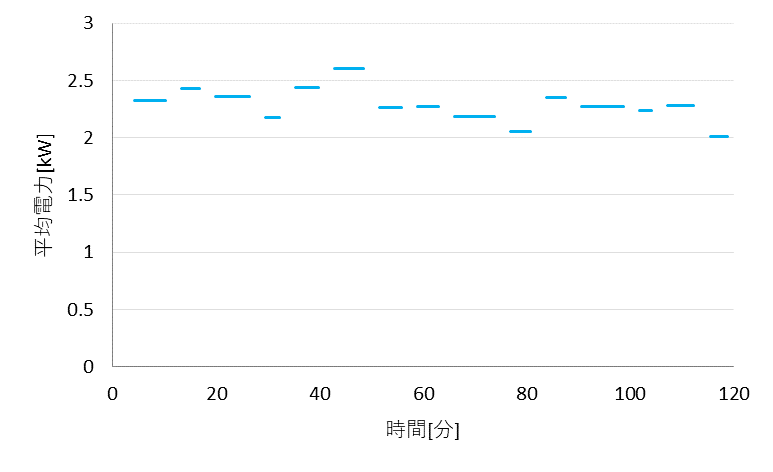
\includegraphics[width=\linewidth]{img/20220803_peak.png}
  \caption{圧縮機発停ごとの平均電力量(8/3)}
  \label{fig:8/3_sato}
\end{figure}

各領域における電力には
大きな違いは見られないが, 平均することにより散水周期による電力の違いを考えられる. それによると, 散水なしの場合では1.47kW, 
10分周期散水の場合は1.33kW, 5分周期散水の場合は1.33kWと求められた. この解析から, 散水前後において電力は9.7\%減少し,
5分, 10分周期の散水では明確な電力低下にはつながらないと考えられる. これは, 室外機の始動運転に電力消費がかかるため,
発停周期が短くなりすぎることは電力低下につながらないのではないかと考えられる.また, 冒頭で述べた各日の電力消費の比較では
測定範囲全体における全電力量を用いた比較を行っているため, 過剰な評価になっていると考えられる. 以上の結果は, 他社による
散水効果(7\%)以上であり, 最適な散水継続時間及び周期はそれぞれ1分, 5~10分であると結論する. 

\subsection{省エネ効果に対する検証}
最後に水道料金も含めた消費コスト低減効果について議論する. 最適な散水条件により, 外気温35℃, 湿度40\%の環境において
電力は9.7\%減少するため, 夏場3か月間, 昼間の6時間効果を発揮したとし、室外機が平均電力量2kWh使用すると仮定すると,
散水なしでは54,000円電気代がかかり,散水ありでは51,300円となり, 夏場に室外機1台当たり2,700円の電気代節約となる.
一方, 散水に用いた水量は, 240mL/minであり, 10分間隔で昼間に散水し続けたとして, 1か月あたり0.2㎥の水道使用量増加になるため,
夏場では180円の増加となる. 以上より, 散水システム導入による省エネ効果は, 室外機1台当たり年間約2,500円である. 自社の場合,
屋上にある室外機は11台であるので, 仮にすべての室外機に散水システムを導入した場合, 年間約27,500円のコストカットが期待される. 
ここで,散水システム導入の初期費用について考える.本研究で用いた散水システムは蛇口による簡易的なシステムのため,費用は材料費のみ
で23,000円程度であった. しかし, 実際に本研究で見出した条件に従って散水を自動化するには, 電磁弁や外気温度センサー, タイマーが必要
となり, 室外機1台当たり材料費で計50,000円になる. さらに工賃や利益も含めると, さらに費用は跳ね上がる.
したがって, 材料費だけでも償却年数に20年かかるため, 1台のみに導入するのは現実的でない. 
しかしながら,複数台の室外機に取り付ける場合は電磁弁に対して複数系統でシステムを組むことにより材料費はより下がると考えられる
ので,イニシャルコスト込みでコストカットを図るには,室外機複数台への導入が現実的である.


\section{結論と今後の課題}
雨天時や長時間散水の計測結果から, 継続的な散水はフィンに水滴が付着することにより熱交換が阻害されることがわかった. 
また, 夏場外気温35℃, 湿度40\%環境下において,散水効果が最も得られるのは,断続的な散水であり,
散水継続時間及び周期はそれぞれ1分, 5~10分であり, 散水なしと比べ, 9.7\%の電力量低減となった.
また,イニシャルコストおよびランニングコストを含めて考えると, 室外機1台のみへの導入は償却年数から
現実的でなく, 複数台導入かつ電磁弁1台に対して複数系統となるなどコストカットの工夫が必要である. 

今後の課題として,スケール対策が挙げられる.本研究での散水では水道水を用いたため,
水道水に含まれる不純物が付着することでスケールと呼ばれるフィン伝熱を阻害するものが
凝縮器に溜まる.
対策としては高圧洗浄機による定期的な清掃や,水の清浄化\cite{thesis3}があるが,
いずれも多大なコストがかかるため,慎重に考える必要がある. 
また,本研究では散水に着目し室外機の熱交換促進を試みたが、他にもさまざまな技術が
研究されているので,それらと比較し,室外機のある様々な環境に適した選定を行うべきか,
評価する必要がある.

%参考文献
\begin{thebibliography}{99}
\bibitem{temp_osaka}
国土交通省, 気象庁, 大阪府 日最高気温の月平均値, 
\url{https://www.data.jma.go.jp/obd/stats/etrn/view/monthly_s3.php?prec_no=62&block_no=47772&year=&month=&day=&view=a2}\vspace{2mm}

\bibitem{temp_osaka2}
George's Web Sites, 大阪府-大阪市の気温に関する統計情報, 
\url{http://www.tvg.ne.jp/george/weather/gw_stat_temp.html?city=oosaka}\vspace{2mm}

\bibitem{temp_osaka3}
A-PLAT 気候変動適応プラットフォーム, 気候変動の観測・予測データ, 大阪府観測データ, 
\url{https://adaptation-platform.nies.go.jp/map/Osaka/index_past.html}\vspace{2mm}

\bibitem{condensing_unit}
三菱電機, 暮らしと設備の業務サイト WIN2K, ビル用マルチエアコン 室外ユニット PUHY-EP335DMG9, 
\url{https://www.mitsubishielectric.co.jp/ldg/wink/ssl/displayProduct.do?pid=317186&ccd=2020121158}\vspace{2mm}

% \bibitem{clie}
% 株式会社クリエ, 高圧カット防止室外機散水装置 トラブルカット, 
% \url{https://c-clie.shop-pro.jp/?pid=134166927}\vspace{2mm}

% \bibitem{daisen}
% ダイセン・メンブレン・ システムズ株式会社, 
% 室外機向け散水システム "E mizu Shower System", 
% \url{https://daicen.com/products/kankyo/emizushower.html}\vspace{2mm}

\bibitem{thesis2}
"エアコン室外機への散水による省エネ効果の実験結果", 
総合技術センター計測・制御技術分野 飯田 仁\vspace{2mm}

\bibitem{夏の節電}
資源エネルギー庁, "2.夏の節電生活の基本を知っておく"\vspace{2mm}

\bibitem{thesis3}
"空調室外機散水システム(Eミズシャワー)による節電・CO2 削減", 
綿部智一, 中塚修志, 
ダイセン・メンブレン・システムズ株式会社技術開発センター\vspace{2mm}

\end{thebibliography}
%
%
%
\end{document}
